\documentclass[a4paper,12pt]{report}

\usepackage{alltt, fancyvrb, url}
\usepackage{graphicx}
\usepackage[utf8]{inputenc}
\usepackage{float}
\usepackage{hyperref}

\usepackage[italian]{babel}

\usepackage[italian]{cleveref}

\usepackage[table]{xcolor}
\usepackage{array}
\usepackage{multirow}
\usepackage{titlesec}

\titleformat{\chapter}[display]
  {\normalfont\bfseries}{}{0pt}{\Huge}


\title{\textbf{Pcd-Assigment01 Report}\\\large Concurrent Boids}
\author{
Bedeschi Federica \\
\textit{0001175655 federica.bedeschi4@studio.unibo.it}\\\\
Pracucci Filippo \\
\textit{0001183555 filippo.pracucci@studio.unibo.it}
}

\date{Anno accademico 2024-2025}



\begin{document}
\maketitle
\newpage

\tableofcontents

% ANALISI
% A brief analysis of the problem, focusing in particular aspects that are relevant from concurrent point of view.
\chapter{Analisi}
\section{Descrizione del problema}
Il problema dei \href{https://en.wikipedia.org/wiki/Boids}{Boids} consiste in una simulazione del comportamento degli stormi di uccelli.
Ogni boid aggiorna la propria posizione in maniera continuativa, solo dopo aver aggiornato la propria velocità in base a quelle degli altri boid. In questo modo si simula il comportamento di gruppo, che può essere condizionato dalle seguenti regole:
\begin{itemize}
    \item separazione: il boid vira al fine di evitare il sovraffollamento locale (dunque si allontana dai boid vicini);
    \item allineamento: il boid vira al fine di allinearsi alle traiettorie di volo dei boid vicini;
    \item coesione: il boid vira al fine di muoversi verso la posizione media (baricentro) dei boid vicini.
\end{itemize}
\section{Visione concorrente}
Dal punto di vista concorrente gli aggiornamenti delle velocità e delle posizioni per ogni boid possono essere fatti concorrentemente. Tuttavia, bisogna tenere conto che tutte le posizioni possono essere aggiornate solo dopo aver aggiornato tutte le velocità, e viceversa.
Analizzando la soluzione sequenziale fornita, è emerso come punto critico, a livello di singolo boid, l'aggiornamento della velocità in quanto nel calcolo dell'allineamento si accede alle velocità dei boid "vicini". Per questo motivo l'accesso a queste ultime viene fatto in mutua esclusione.\\
A livello di interfaccia grafica, l'aggiornamento della vista deve essere eseguito a seguito dell'aggiornamento di tutte le posizioni dei boid.

% DESIGN E ARCHITETTURA
% A description of the adopted design, the strategy and architecture.
% A description of the behaviour of the system using one or multiple Petri Nets, choosing the propor level of abstraction.
\chapter{Design e architettura}
Abbiamo optato per un'architettura che seguisse il pattern \textit{MVC}, quindi con un \textit{Controller} che si occupasse di mettere in comunicazione il \textit{Model} con la \textit{View}. Ogni versione utilizza un Controller equivalente, modificando esclusivamente il metodo di avvio della simulazione.
I Controller sfruttano due monitor per notificare i componenti attivi degli eventi di sospensione ed interruzione scaturiti dalla View.
\section{Multithreaded}
\label{sec:multithreaded}
Abbiamo creato due tipi di worker, un \textit{ComputeWorker} che si occupa di tutta la computazione riguardante i boid, e un \textit{GUIWorker} che si occupa di aggiornare l'interfaccia grafica. Viene istanziato un numero di ComputeWorker uguale al numero di core presenti nella macchina sottostante, consentendo di sfruttare appieno tutte le risorse dell'architettura. Al contrario viene istanziato un singolo GUIWorker.\\
Al fine di bilanciare il lavoro dei ComputeWorker, ad ognuno viene affidata una porzione dei boid totali.
Per effettuare la sincronizzazione tra i worker abbiamo creato una barriera ciclica, della quale utilizziamo due istanze, una per attendere il completamento degli aggiornamenti delle velocità, ed una seconda per aspettare la terminazione degli aggiornamenti delle posizioni. Entrambe le barriere vengono utilizzate sia dai ComputeWorker che dal GUIWorker.
\subsection{Rete di Petri}
\label{sec:petri-net-multithreaded}
La rete di Petri in \Cref{fig:petri-net-multithreaded} descrive il comportamento del sistema, ovvero si compone di due attività, una per i ComputeWorker ed una per il GUIWorker. La prima gestisce un numero di token pari al numero di istanze di ComputeWorker create, cioè il numero di core disponibili (N); mentre la seconda gestisce un unico token. L'attività del GUIWorker si sincronizza con quella dei ComputeWorker in corrispondenza delle due barriere posizionate in seguito all'aggiornamento delle velocità e delle posizioni.
\begin{figure}[H]
    \centering
    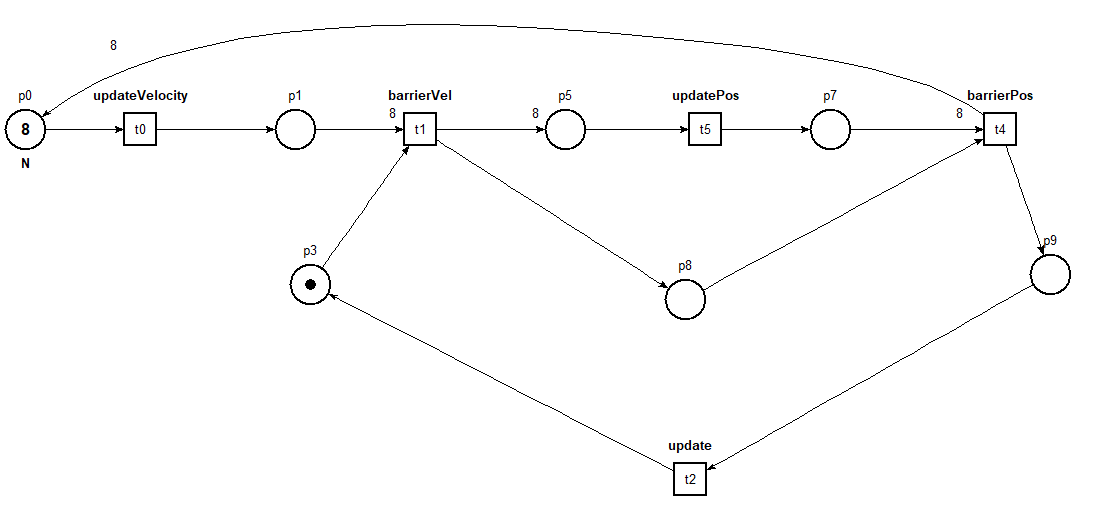
\includegraphics[width=\linewidth]{figures/multithreaded.png}
    \caption{\centering Rete di Petri - multithreaded \newline \textit{Ogni 8 presente in figura rappresenta in realtà gli N ComputeWorker utilizzati.}}
    \label{fig:petri-net-multithreaded}
\end{figure}
\section{Task-based}
Il comportamento complessivo viene gestito da un \textit{MasterWorker}, il quale si compone di un \textit{Executor}, che manda in esecuzione nei momenti opportuni tre tipi di task diversi:
\begin{itemize}
    \item \textit{UpdateVelocityTask}: si occupa di aggiornare la velocità di un singolo boid;
    \item \textit{UpdatePositionTask}: si occupa di aggiornare la posizione di un singolo boid;
    \item \textit{UpdateGUITask}: si occupa di aggiornare l'interfaccia grafica, dopo aver calcolato il frame rate attuale.
\end{itemize}
Ad ogni iterazione viene eseguito un numero di UpdateVelocityTask e UpdatePositionTask pari al numero di boids ed un singolo UpdateGUITask.\\
La sincronizzazione viene gestita tramite il meccanismo dei \textit{Future}, ovvero fornendo all'Executor i task delle posizioni solo dopo aver ottenuto tutti i risultati relativi ai task delle velocità, e viceversa; mentre l'UpdateGUITask viene eseguito concorrentemente a quelli delle velocità ed il risultato che fornisce corrisponde al tempo che viene utilizzato per calcolare il frame rate.
\subsection{Rete di Petri}
La rete di Petri in \Cref{fig:petri-net-task-based} descrive il comportamento del sistema, evidenziando i punti di sincronizzazione, come descritto sopra, e l'esecuzione concorrente dell'UpdateGUITask con i task delle velocità. I token corrispondono al numero di task eseguiti ad ogni iterazione.
Differentemente da quanto descritto nella \cref{sec:petri-net-multithreaded} gli UpdatePositionTask hanno un flusso di controllo separato rispetto agli UpdateVelocityTask.
\begin{figure}[H]
    \centering
    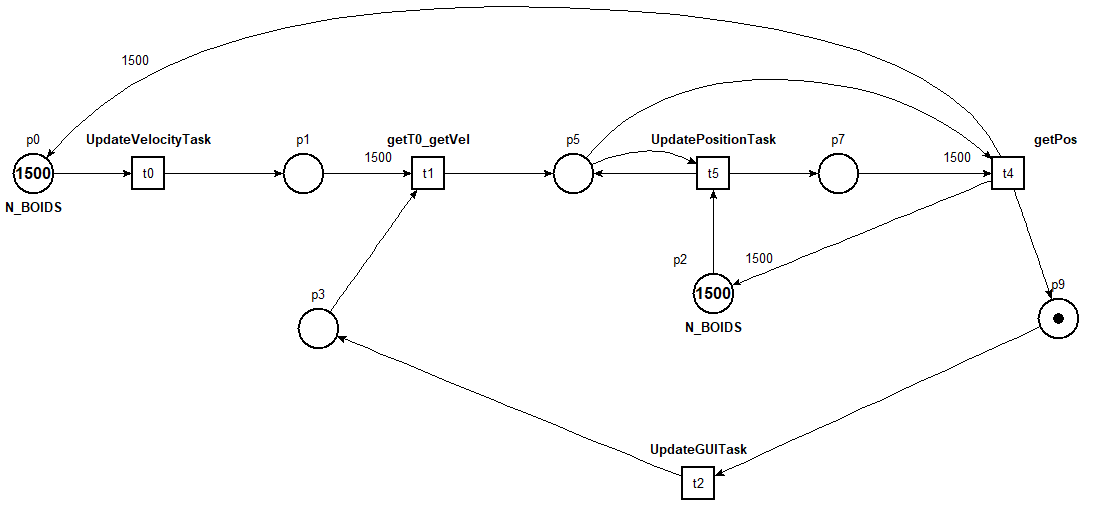
\includegraphics[width=\linewidth]{figures/tasks.png}
    \caption{\centering Rete di Petri - task-based \newline \textit{Ogni 1500 presente in figura rappresenta in realtà gli N\_BOIDS gestiti.}}
    \label{fig:petri-net-task-based}
\end{figure}
\section{Virtual threads}
Abbiamo creato due tipi di worker, un \textit{ComputeWorker} che si occupa di tutta la computazione riguardante un singolo boid, e un \textit{GUIWorker} che si occupa di aggiornare l'interfaccia grafica. Ogni worker è gestito da un singolo \textit{Virtual Thread}, quindi complessivamente sono presenti un numero di Virtual Thread pari al numero di boids ed in aggiunta uno per il GUIWorker. La sincronizzazione viene gestita analogamente al caso \textit{Multithreaded}, come descritto nella \cref{sec:multithreaded}.
\subsection{Rete di Petri}
La rete di Petri in \Cref{fig:petri-net-virtual-threads} descrive il comportamento del sistema, ovvero si compone di due attività, una per i ComputeWorker ed una per il GUIWorker. La prima gestisce un numero di token pari al numero di istanze di ComputeWorker create, cioè il numero di boids (N\_BOIDS); mentre la seconda gestisce un unico token. L'attività del GUIWorker si sincronizza con quella dei ComputeWorker in corrispondenza delle due barriere posizionate in seguito all'aggiornamento delle velocità e delle posizioni.
\begin{figure}[H]
    \centering
    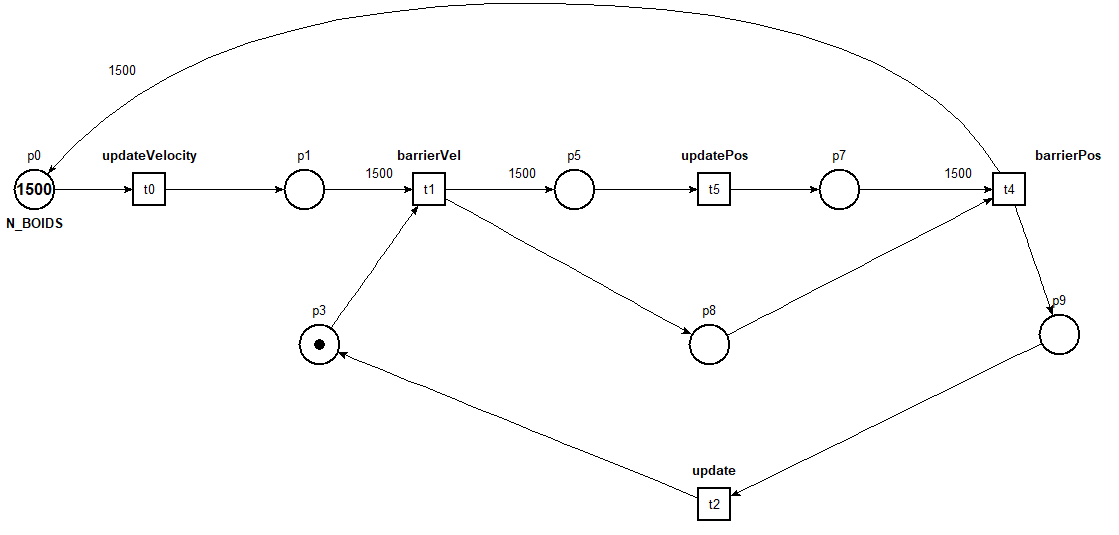
\includegraphics[width=\linewidth]{figures/virtualthreads.png}
    \caption{\centering Rete di Petri - virtual threads \newline \textit{Ogni 1500 presente in figura rappresenta in realtà il numero di ComputeWorker (equivalente agli N\_BOIDS utilizzati).}}
    \label{fig:petri-net-virtual-threads}
\end{figure}

% TEST PERFORMANCE
% Performance tests, to analyse and discuss the performance of the programs (for each version) compared to the sequential version
\chapter{Test performance}
Per valutare le performance delle varie versioni in relazione a quella sequenziale, abbiamo misurato il throughput, ovvero il tempo impiegato per effettuare un'iterazione. Per aver valori più consistenti abbiamo preso in considerazione 500 iterazioni e abbiamo calcolato la media.\\
Per ogni versione abbiamo ripetuto le misurazioni al variare del numero di boid e del numero di thread.
Nello specifico, la versione sequenziale è rappresentata in ogni grafico dalla curva indicata con un thread, mentre le altre rappresentano la versione concorrente al variare del numero di thread.\\
I valori ottenuti con 9 thread sono evidenziati in quanto rappresentano il valore teoricamente ottimale, ovvero $N\_core + 1$, considerando che l'architettura utilizzata per effettuare i test presenta un processore ad 8 core.\\
Per ogni versione riportiamo i calcoli dello speedup e dell'efficienza, secondo le formule:
\begin{itemize}
    \item Speedup: $S = \frac{T_1}{T_N}$, dove $T_1$ indica il throughput del caso sequenziale e $T_N$ il throughput del caso concorrente con $N$ thread;
    \item Efficienza: $E = \frac{S}{N}$, dove $S$ indica lo speedup e $N$ il numero di thread.
\end{itemize}

\section{Multithreaded}
\begin{figure}[H]
    \centering
    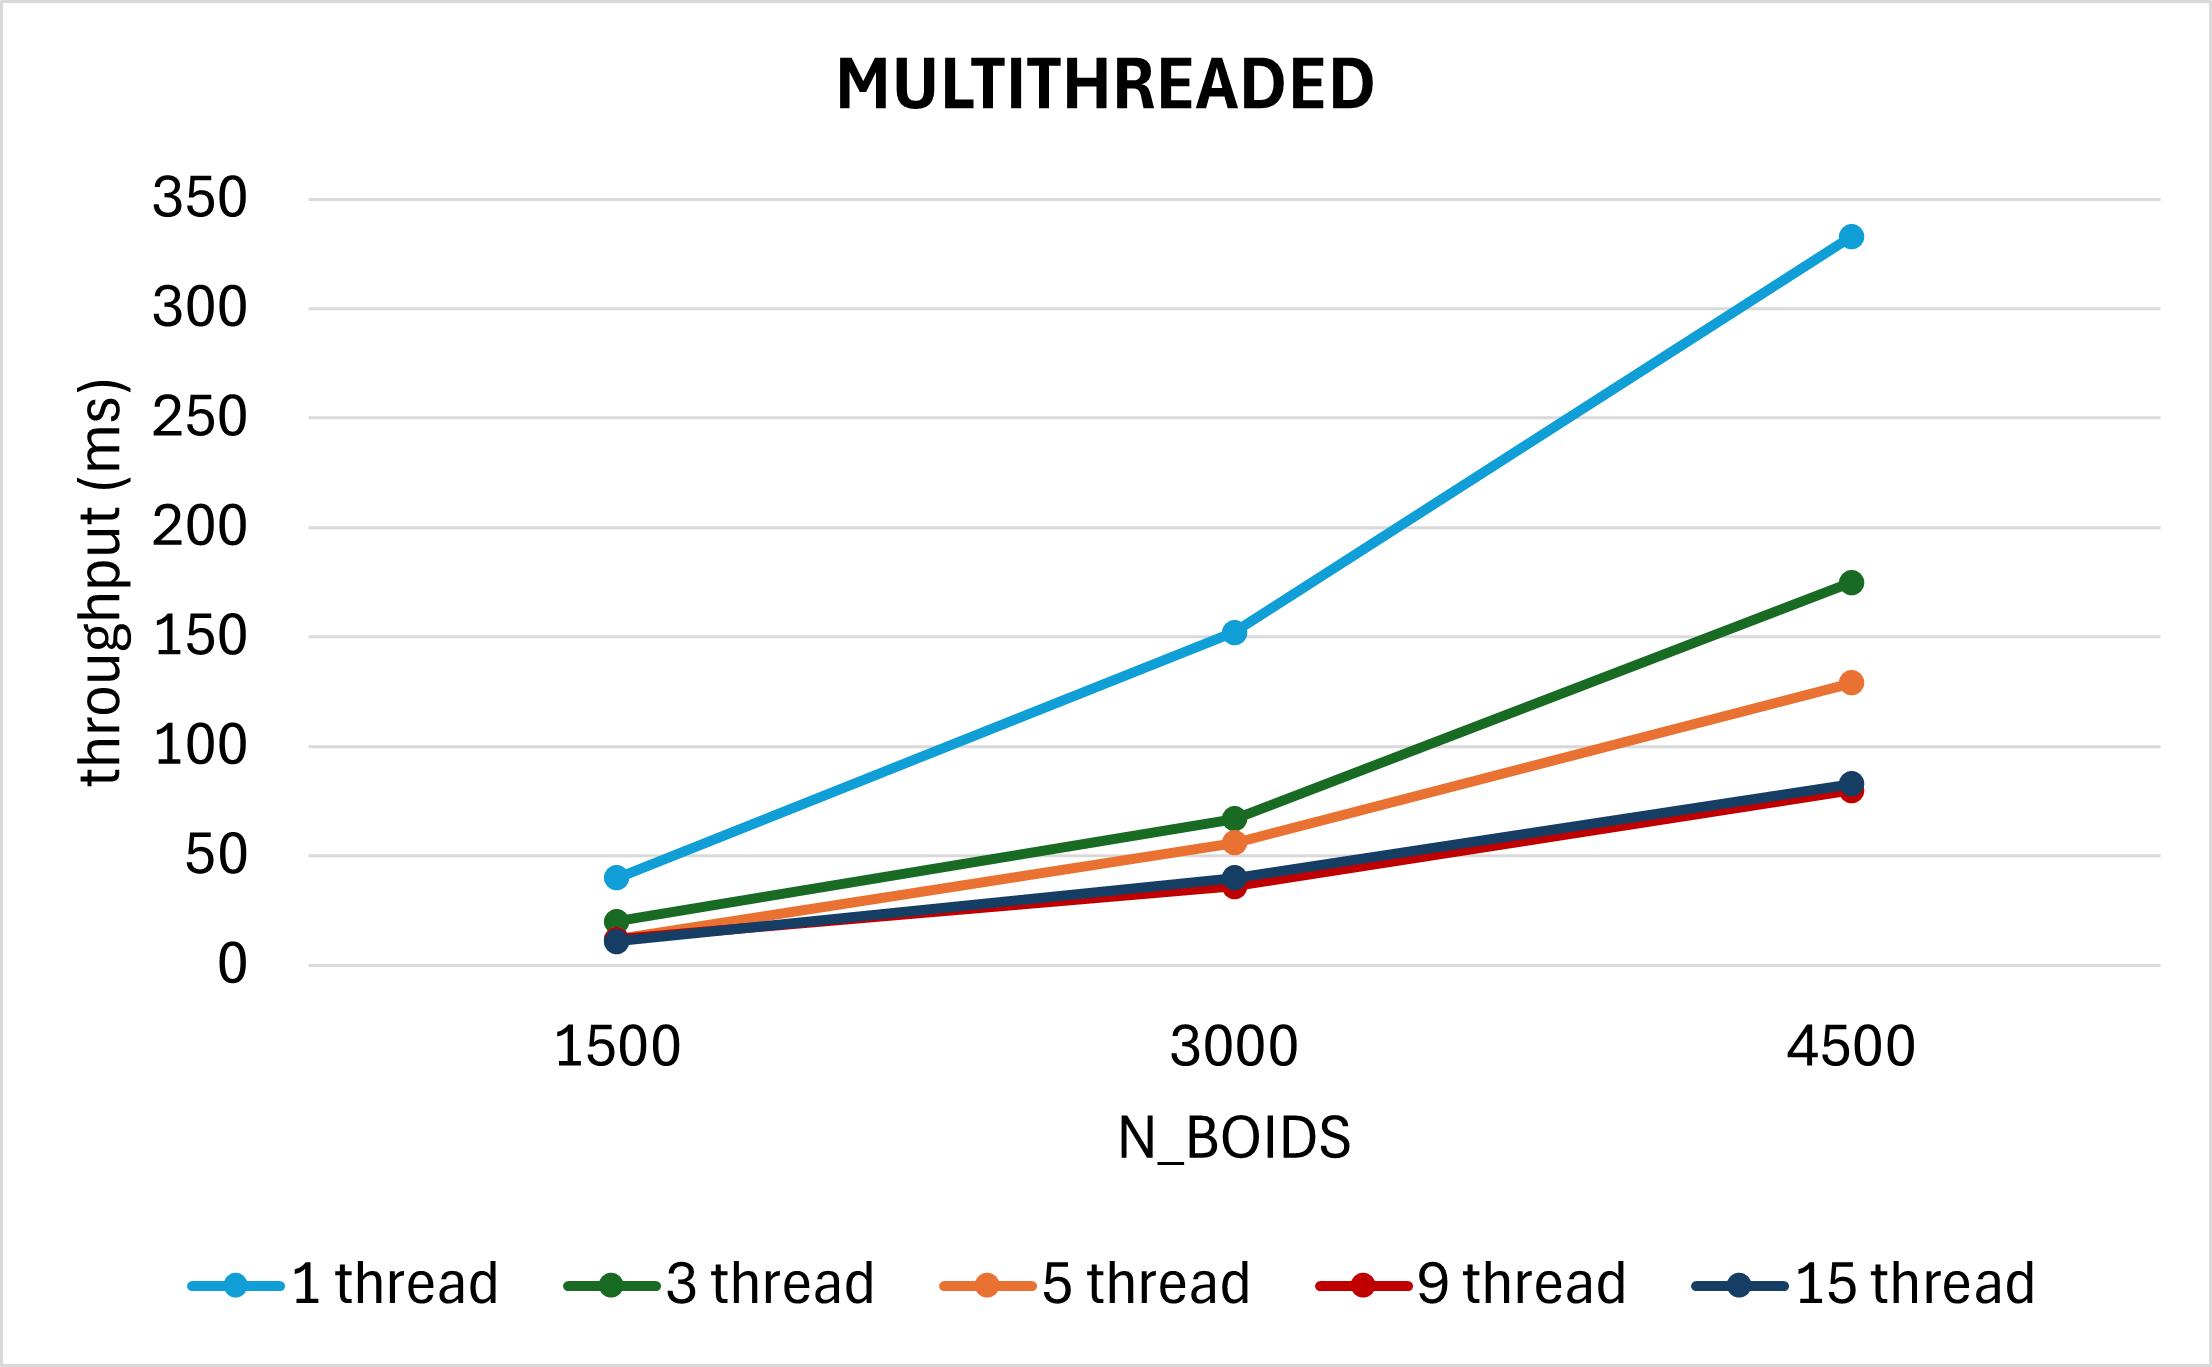
\includegraphics[width=\linewidth]{figures/multithreaded_test.png}
    \caption{\centering Throughput test - multithreaded}
    \label{fig:throughput-test-multithreaded}
\end{figure}

\begin{table}[!htb]
    \renewcommand{\arraystretch}{1.5}
    \centering
    \begin{tabular}{|l|c|ccc|}
        \hline
        \multicolumn{1}{|c|}{}      & \multirow{2}{*}{N\_THREADS} & \multicolumn{3}{c|}{N\_BOIDS}                                \\ \cline{3-5}
        \multicolumn{1}{|c|}{}      &                     & \multicolumn{1}{c|}{1500} & \multicolumn{1}{c|}{3000} & 4500 \\ \hline
        \multirow{4}{*}{Speedup}    & 15                  & \multicolumn{1}{c|}{3.64} & \multicolumn{1}{c|}{3.80} & 4.01 \\ \cline{2-5} 
         & \textbf{9}                    & \multicolumn{1}{c|}{\textbf{3.33}} & \multicolumn{1}{c|}{\textbf{4.22}} & \textbf{4.16} \\ \cline{2-5} 
         & 5 & \multicolumn{1}{c|}{3.33} & \multicolumn{1}{c|}{2.71} & 2.58 \\ \cline{2-5} 
         & 3 & \multicolumn{1}{c|}{2.00} & \multicolumn{1}{c|}{2.27} & 1.90 \\ \hline
        \multirow{4}{*}{Efficienza} & 15                  & \multicolumn{1}{c|}{0.24} & \multicolumn{1}{c|}{0.25} & 0.27 \\ \cline{2-5} 
         & \textbf{9}   & \multicolumn{1}{c|}{\textbf{0.37}} & \multicolumn{1}{c|}{\textbf{0.47}} & \textbf{0.46} \\ \cline{2-5} 
         & 5            & \multicolumn{1}{c|}{0.67} & \multicolumn{1}{c|}{0.54} & 0.52 \\ \cline{2-5} 
         & 3            & \multicolumn{1}{c|}{0.67} & \multicolumn{1}{c|}{0.76} & 0.63 \\ \hline
    \end{tabular}
    \caption{Misure performance - multithreaded}
    \label{table:performance_multithreaded}
\end{table}

\section{Task-based}
\begin{figure}[H]
    \centering
    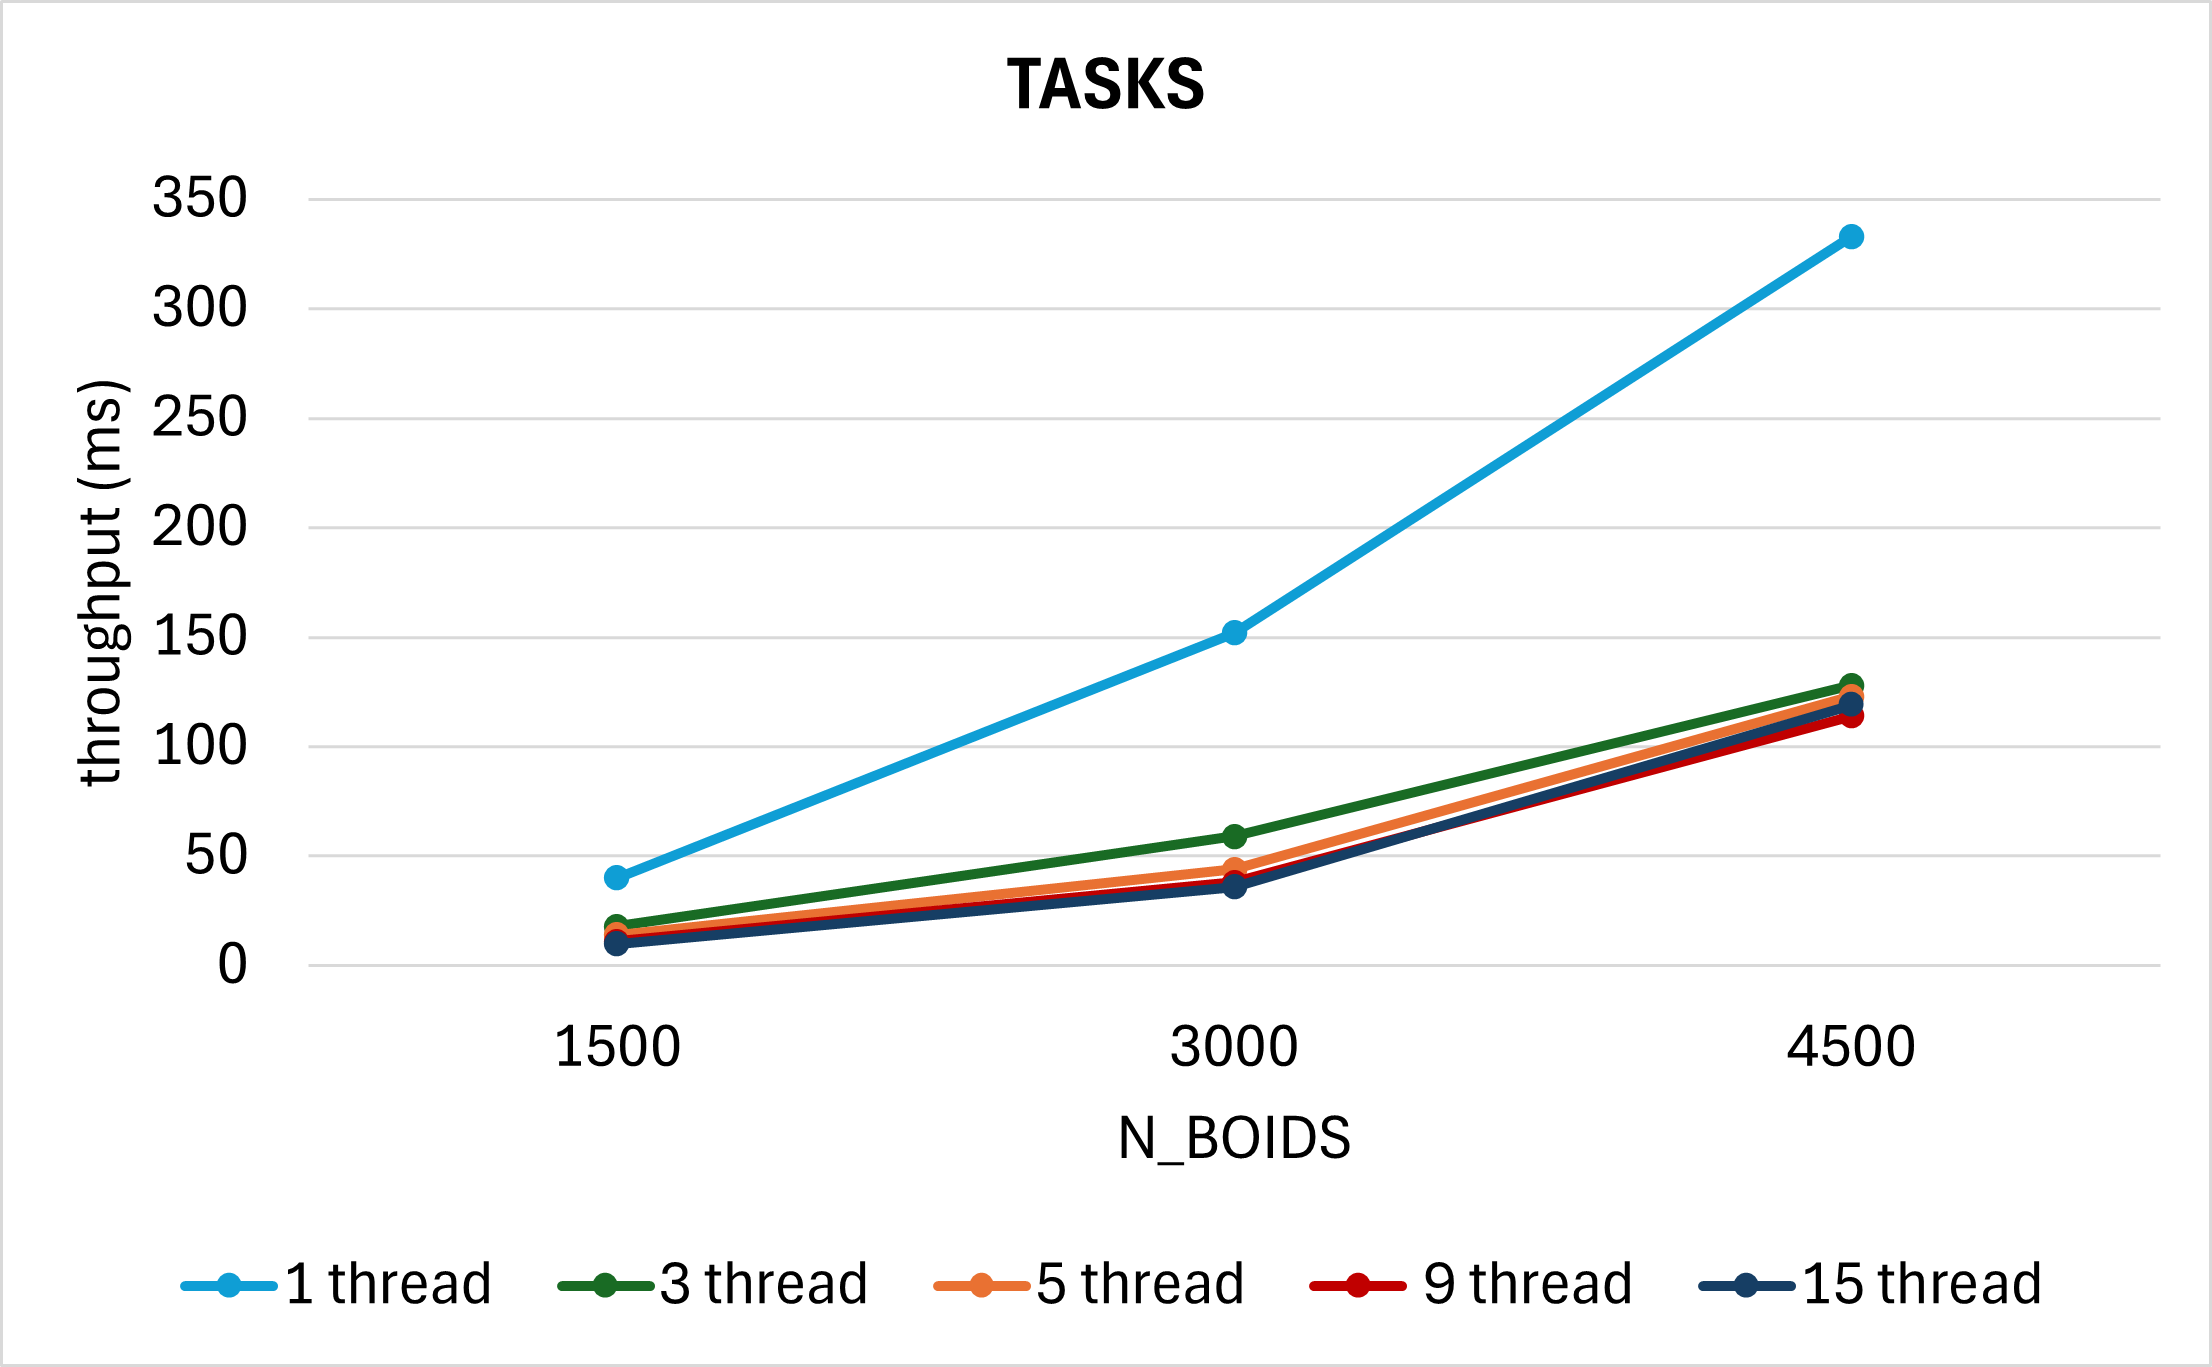
\includegraphics[width=\linewidth]{figures/tasks_test.png}
    \caption{\centering Throughput test - task-based}
    \label{fig:throughput-test-tasks}
\end{figure}

\begin{table}[!htb]
    \renewcommand{\arraystretch}{1.5}
    \centering
    \begin{tabular}{|l|c|ccc|}
        \hline
        \multicolumn{1}{|c|}{}      & \multirow{2}{*}{N\_THREADS} & \multicolumn{3}{c|}{N\_BOIDS}                                \\ \cline{3-5}
        \multicolumn{1}{|c|}{}      &                     & \multicolumn{1}{c|}{1500} & \multicolumn{1}{c|}{3000} & 4500 \\ \hline
        \multirow{4}{*}{Speedup}    & 15                  & \multicolumn{1}{c|}{4.00} & \multicolumn{1}{c|}{4.22} & 2.80 \\ \cline{2-5} 
         & \textbf{9}                    & \multicolumn{1}{c|}{\textbf{3.64}} & \multicolumn{1}{c|}{\textbf{4.00}} & \textbf{2.92} \\ \cline{2-5}
         & 5 & \multicolumn{1}{c|}{2.86} & \multicolumn{1}{c|}{3.45} & 2.71 \\ \cline{2-5} 
         & 3 & \multicolumn{1}{c|}{2.22} & \multicolumn{1}{c|}{2.58} & 2.60 \\ \hline
        \multirow{4}{*}{Efficienza} & 15                  & \multicolumn{1}{c|}{0.27} & \multicolumn{1}{c|}{0.28} & 0.19 \\ \cline{2-5} 
         & \textbf{9}   & \multicolumn{1}{c|}{\textbf{0.24}} & \multicolumn{1}{c|}{\textbf{0.25}} & \textbf{0.27} \\ \cline{2-5}
         & 5            & \multicolumn{1}{c|}{0.57} & \multicolumn{1}{c|}{0.69} & 0.54 \\ \cline{2-5} 
         & 3            & \multicolumn{1}{c|}{0.74} & \multicolumn{1}{c|}{0.86} & 0.87 \\ \hline
    \end{tabular}
    \caption{Misure performance - task-based}
    \label{table:performance_task-based}
\end{table}

\section{Virtual threads}
In questa versione abbiamo preso in considerazione solo un numero di thread pari a 9, in quanto non siamo riusciti a modificare il numero di platform thread.

\begin{figure}[H]
    \centering
    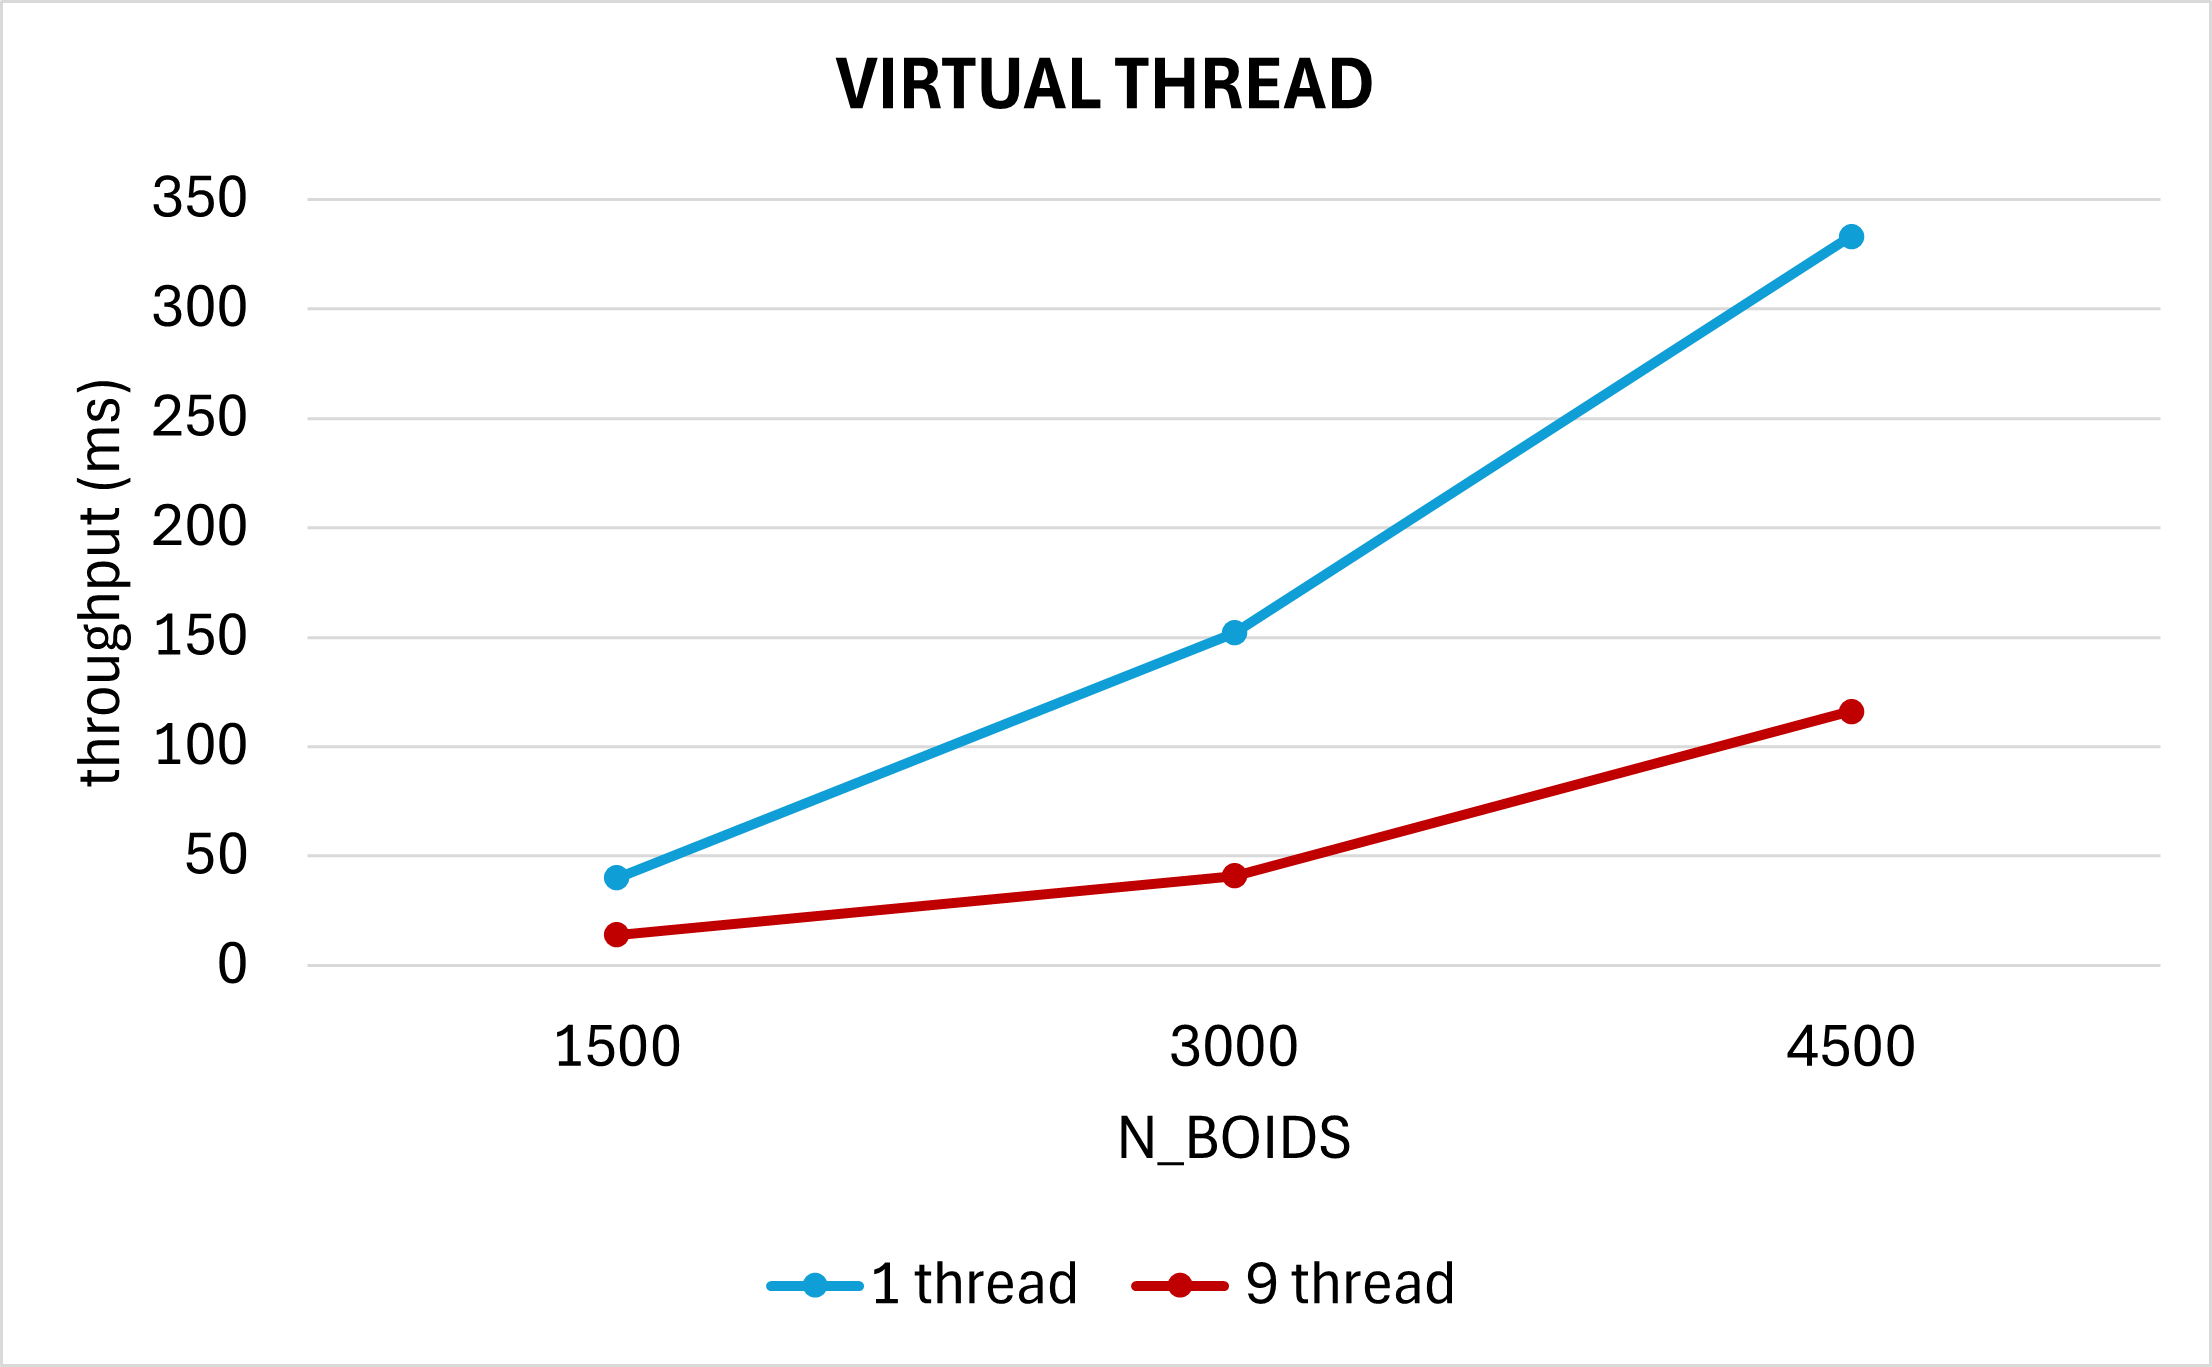
\includegraphics[width=\linewidth]{figures/virtualthread_test.png}
    \caption{\centering Throughput test - virtual threads}
    \label{fig:throughput-test-virtual-threads}
\end{figure}

\begin{table}[!htb]
    \renewcommand{\arraystretch}{1.5}
    \centering
    \begin{tabular}{|l|c|ccc|}
        \hline
        \multicolumn{1}{|c|}{} & \multirow{2}{*}{N\_THREADS} & \multicolumn{3}{c|}{N\_BOIDS}                                \\ \cline{3-5} 
        \multicolumn{1}{|c|}{} &                          & \multicolumn{1}{c|}{1500} & \multicolumn{1}{c|}{3000} & 4500 \\ \hline
        Speedup                & 9                        & \multicolumn{1}{c|}{2.86} & \multicolumn{1}{c|}{3.71} & 2.87 \\ \hline
        Efficienza             & 9                        & \multicolumn{1}{c|}{0.32} & \multicolumn{1}{c|}{0.41} & 0.32 \\ \hline
    \end{tabular}
    \caption{Misure performance - virtual threads}
    \label{table:performance_virtual_threads}
\end{table}

% Speedup: S = T1 / TN
% Efficiency: E = S / N

% sequential:
% 1500 -> 40 ms; 3000 -> 152 ms; 4500 -> 333 ms
% multithreaded:
% 14+1 thread:1500 -> 8 ms;  3000 -> 25-29 ms; 4500 -> 60-86 ms
% 14+1 thread:1500 -> 11 ms; 3000 -> 40 ms; 4500 -> 83 ms
% 8+1 thread: 1500 -> 12 ms; 3000 -> 36 ms; 4500 -> 80 ms
%       oggi: 1500 -> 10 ms; 3000 -> 30 ms; 4500 -> 56-80 ms
% 4+1 thread: 1500 -> 12 ms; 3000 -> 56 ms; 4500 -> 129 ms
% 2+1 thread: 1500 -> 20 ms; 3000 -> 67 ms; 4500 -> 175 ms
%   speedup:
% 14+1 thread:1500 -> 3.64; 3000 -> 3.80; 4500 -> 4.01
% 8+1 thread: 1500 -> 3.33; 3000 -> 4.22; 4500 -> 4.16
% 4+1 thread: 1500 -> 3.33; 3000 -> 2.71; 4500 -> 2.58
% 2+1 thread: 1500 -> 2; 3000 -> 2.27; 4500 -> 1.90
%   efficienza:
% 14+1 thread:1500 -> 0.24; 3000 -> 0.25; 4500 -> 0.27
% 8+1 thread: 1500 -> 0.37; 3000 -> 0.47; 4500 -> 0.46
% 4+1 thread: 1500 -> 0.67; 3000 -> 0.54; 4500 -> 0.52
% 2+1 thread: 1500 -> 0.67; 3000 -> 0.76; 4500 -> 0.63
% tasks:
% 15 thread:  1500 -> 10 ms; 3000 -> 36 ms; 4500 -> 119 ms
% 9 thread:   1500 -> 11 ms; 3000 -> 38 ms; 4500 -> 114 ms
% 5 thread:   1500 -> 14 ms; 3000 -> 44 ms; 4500 -> 123 ms
% 3 thread:   1500 -> 18 ms; 3000 -> 59 ms; 4500 -> 128 ms
% virtual threads:
% 9 thread:   1500 -> 14 ms; 3000 -> 41 ms; 4500 -> 116 ms oggi range 82->97ms
% 9 thread #2:1500 -> 13 ms; 3000 -> 39 ms; 4500 -> 81->90ms
% 5 thread;   1500 -> 14 ms; 3000 -> 50 ms; 4500 -> 106 ms X
% 3 thread:   1500 -> 16 ms; 3000 -> 43 ms; 4500 -> 114 ms X

% random example
% 1 thread:  74172 ms
% 2 threads: 41400 ms  speedup = 74172 / 41400 = 1.79   efficiency = 1.79 / 2 = 0.90
% 8 threads: 34894 ms  speedup = 74172 / 34894 = 2.13   efficiency = 2.13 / 8 = 0.27

%CONCLUSIONI
% Verification of the program (a model of it) using JPF. For this point, only the Java multithreaded programming version may be considered.
\chapter{Conclusioni}
Per quanto riguarda le performance si può notare come le varie versioni concorrenti scalino correttamente all'aumentare del numero di boid e in relazione al numero di thread. Il miglioramento delle prestazioni, come ci si poteva aspettare, però ha un limite in corrispondenza di un numero di thread pari a $N\_core + 1$, quindi nel nostro caso 9 thread, che corrisponde al valore teoricamente ottimale; questo lo si nota nei grafici e nelle tabelle in corrispondenza dei valori ottenuti utilizzando 15 thread. Inoltre, come evidenziato dai grafici e dai valori dello speedup, c'è un miglioramento significativo nelle prestazioni delle versioni concorrenti rispetto a quelle della versione sequenziale.\\
Abbiamo controllato la correttezza del nostro modello multithreaded tramite il tool JPF utilizzando una versione semplificata con le sole barriere per la sincronizzazione ed utilizzando un numero di iterazioni predefinito. Da questo controllo non è emerso nessun errore.

\end{document}
